\documentclass[
    a4paper,
    12pt,
]{article}
\usepackage{amsmath, amsthm, amsfonts, amssymb}
\usepackage{microtype}
\usepackage{geometry}
\usepackage{booktabs}
\usepackage{graphicx, tikz}
\usepackage{caption}
\usepackage{subcaption}
% \geometry{margin=1in}
\usepackage{comment}

\usepackage{hyperref}
\usepackage[capitalise]{cleveref}
\usepackage{xcolor}
\hypersetup{ % this is just my personal choice, feel free to change things
    colorlinks,
    linkcolor={red!50!black},
    citecolor={blue!50!black},
    urlcolor={blue!80!black},
}

\usepackage{cancel}
\usepackage{mathtools}

\usepackage{enumerate}
\usepackage{enumitem}

\DeclarePairedDelimiter\abs{\lvert}{\rvert}%
\DeclarePairedDelimiter\norm{\lVert}{\rVert}%

% 1. Define a ‘breaktheorem’ style that:
%    - Uses bold for the theorem heading,
%    - Puts (number + optional note) on the *same line*,
%    - Forces a line-break before the body text.
\makeatletter
\newtheoremstyle{breaktheorem}%
{\topsep}{\topsep}%   % Above/below space
{
    \addtolength{\@totalleftmargin}{3.5em}
    \addtolength{\linewidth}{-3.5em}
    \parshape 1 3.5em \linewidth % chktex 1
    \itshape
}% body font
{}%                   % Indent
{\bfseries}%          % Head font
{}%                  % Punctuation after theorem head
{ }%           % Space (or line break) after theorem head
{\thmname{#1} \thmnote{#3}}
\makeatother
%   #1 = Theorem name ("Theorem")
%   #2 = Theorem number ("4.3")
%   #3 = The optional note (e.g., "Cea's lemma")

% 2. Tell amsthm to use this style for Theorem.
\theoremstyle{breaktheorem}
\newtheorem{theorem}{Theorem}[section]

\numberwithin{equation}{section}

\title{
    MAT4170\\
    \small{Exercises for Spline Methods}
}
\author{August Femtehjell}
\date{Spring 2025}

\begin{document}

\maketitle

\tableofcontents

\begin{abstract}
    This document contains my summary for the course MAT4170 -- Spline Methods, taught at the University of Oslo in the spring of 2025, in preperation for the final oral exam. % chktex 8
    This summary is based on the \href{https://www.uio.no/studier/emner/matnat/math/MAT4170/v25/undervisningsmateriale/spline_notes.pdf}{lecture notes} for the course, draft dated 25th of March, 2025.
    The code for everything, as well as this document, can be found at my GitHub repository: \url{https://github.com/augustfe/MAT4170}.
\end{abstract}

\section{Bernstein polynomials}

A Bernstein polynomial denoted $B_i^d$ is defined by
\begin{equation}
    B_i^d(x) = \binom{d}{i} x^i (1 - x)^{d - i},
\end{equation}
where $d$ is the degree of the polynomial, and $i$ is the index of the polynomial.
These polynomials satisfy a number of interesting properties.

Firstly, they are all non-negative on the interval $[0, 1]$.
We can clearly see this as then both $x \geq 0$ and $1 - x \geq 0$ (and of course the binomial coefficient as well).
In addition, for all $x \in \mathbb{R}$ we have that
\begin{equation}
    \sum_{i = 0}^{d} B_i^d(x) = 1,
\end{equation}
and the polynomials therefore form a partition of unity.
We can see this by noting
\begin{equation}
    1
    = 1^d
    = (x + (1 - x))^d
    = \sum_{i = 0}^{d} \binom{d}{i} x^i (1 - x)^{d - i}
    = \sum_{i = 0}^{d} B_i^d(x),
\end{equation}
by the binomial theorem.

In order to compute the value of a Bernstein polynomial efficiently, we note that
\begin{equation}
    \binom{d}{i} = \binom{d - 1}{i - 1} + \binom{d - 1}{i},
\end{equation}
most easily recalled by thinking about Pascals triangle.
With this, we have that
\begin{align*}
    B_{i}^{d}
    &= \binom{d}{i} x^i (1 - x)^{d - i} \\
    &= \left(\binom{d - 1}{i - 1} + \binom{d - 1}{i}\right) x^i (1 - x)^{d - i} \\
    &= x \binom{d - 1}{i - 1} x^{i - 1} (1 - x)^{(d - 1) - (i - 1)} + (1 - x) \binom{d - 1}{i} x^i (1 - x)^{(d - 1) - i} \\
    &= x B_{i - 1}^{d - 1}(x) + (1 - x)B_{i}^{d - 1},
\end{align*}
forming the basis for de Casteljau's algorithm.


\section{Divided differences}
Central to our definition of B-splines is divided differences.
One simple definition of a divided difference, denoted
\begin{equation}
    [x_0, x_1, \dots, x_k]f,
\end{equation}
is that it is the leading coefficient of the polynomial which interpolates $f$ at the points $x_0, x_1, \dots, x_k$.
This is a rather cryptic definition, however it lends itself some nice properties.

\subsection{Distinct points}
If the points $x_i$ are distinct, we have that the polynomial $p$ is the Lagrange polynomial.
As such, we find that
\begin{equation}
    [x_i]f = f(x_i).
\end{equation}
For $k \geq 1$, we can define the polynomial recursively.
Let $p_0$ be the interpolating polynomial at $x_0, x_1, \dots, x_{k - 1}$ and $p_1$ the one at $x_1, x_2, \dots, x_k$.
Then we can write
\begin{equation}
    p(x) = \frac{x_k - x}{x_k - x_0} p_0(x) + \frac{x - x_0}{x_k - x_0} p_0(x).
\end{equation}
From this, we deduce that
\begin{equation}
    [x_0, x_1, \dots, x_k]f = \frac{
        [x_1, x_2, \dots, x_k]f
        - [x_0, x_1, \dots, x_{k - 1}]f
    }{x_k - x_0},
\end{equation}
such that for instance
\begin{equation}
    [x_0, x_1]f
    = \frac{[x_1]f - [x_0]f}{x_1 - x_0}
    = \frac{f(x_1) - f(x_0)}{x_1 - x_0}.
\end{equation}

\subsection{Repeated points}
When there are repeated points, we utilize the Taylor expansion in order to define
\begin{equation}
    [x_0, \dots, x_k]f = [\underbrace{x_0, \dots, x_0}_{k+1}]f = \frac{f^{(k)}(x_0)}{k!}.
\end{equation}

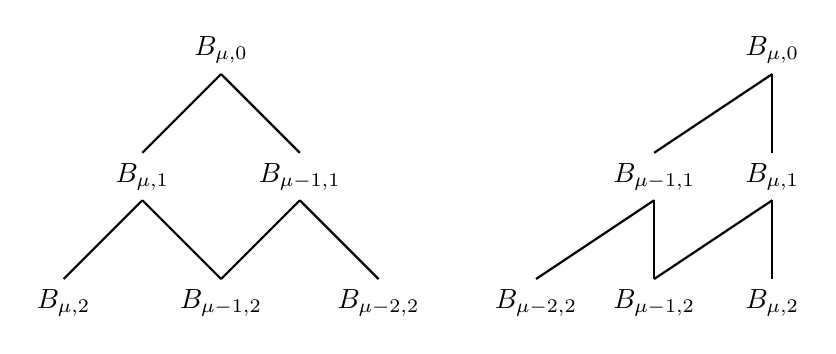
\begin{tikzpicture}[>=stealth, thick]

    % A box for "XAI" on the left
    \node (init) at (0,0) {$B_{\mu, 0}$};

    \draw (init.south) -- ++(-1, -1) coordinate (l);
    \draw (init.south) -- ++(1, -1) coordinate (r);

    \node[anchor=north] (l1) at (l) {$B_{\mu, 1}$};
    \node[anchor=north] (r1) at (r) {$B_{\mu - 1, 1}$};

    \draw (l1.south) -- ++(-1, -1) coordinate (l2);
    \draw (l1.south) -- ++(1, -1) coordinate (lr2);
    \draw (r1.south) -- (lr2);
    \draw (r1.south) -- ++(1, -1) coordinate (r2);

    \node[anchor=north] (l2) at (l2) {$B_{\mu, 2}$};
    \node[anchor=north] (lr2) at (lr2) {$B_{\mu - 1, 2}$};
    \node[anchor=north] (r2) at (r2) {$B_{\mu - 2, 2}$};

    \node (alt) at (7, 0) {$B_{\mu, 0}$};

    \draw (alt.south) -- ++(-1.5, -1) coordinate (altl);
    \draw (alt.south) -- ++(0, -1) coordinate (altr);

    \node[anchor=north] (altl1) at (altl) {$B_{\mu-1, 1}$};
    \node[anchor=north] (altr1) at (altr) {$B_{\mu, 1}$};

    \draw (altl1.south) -- ++(-1.5, -1) coordinate (altl2);
    \draw (altl1.south) -- ++(0, -1) coordinate (altr2);
    \draw (altr1.south) -- (altr2);
    \draw (altr1.south) -- ++(0, -1) coordinate (altr3);

    \node[anchor=north] (altl2) at (altl2) {$B_{\mu - 2, 2}$};
    \node[anchor=north] (altr2) at (altr2) {$B_{\mu - 1, 2}$};
    \node[anchor=north] (altr3) at (altr3) {$B_{\mu, 2}$};
\end{tikzpicture}

\end{document} % chktex 17